\chapter{Algorytm równoległy\label{chap:algorytm}}

Niniejszy rozdział można traktować, jako uzupełnienie rozdziału~\ref{chap:teoria}, w którym to dokonano opisu podstaw teoretycznych wraz z dwoma wiodącymi algorytmami do odkrywania reguł asocjacyjnch. W ramach niniejszej pracy opracowany został algorytm równoległy, oparty na algorytmie opisanym w sekcji~\ref{sec:apriori}.

Wcześniej zaś przedstawione zostanie zastosowanie algorytmu Apriori (opisanego w części~\ref{apriori:section} pracy), w którym wykorzystane zostały funkcje dostarczone przez najnowsze wydanie frameworka .NET. 

W rozdziale tym wykorzystywane są oznaczenia wprowadzone w rozdziale~\ref{chap:teoria}.

\section{Algorytm ParallelApriori\label{sec:papriori}}
Pierwszym algorytmem wykorzystującym możliwości procesorów równoległych jest ParallelApriori - stworzony na potrzeby niniejszej pracy. 

Jak wspomniano już wcześniej, zagadnienie odkrywania reguł asocjacyjnych można podzielić na dwa etapy~\cite{Problem:Statement}:
\begin{enumerate}
	\item Odkrywanie zbiorów częstych, których wartość wsparcia jest wyższa od wartości $minsup$.
	\item Generowanie reguł asocjacyjnych na podstawie znalezionych zbiorów częstych.

	Na tym etapie możliwe jest tworzenie reguł, w których w zbiorze \emph{poprzedników} ($X$ z oznaczeń z definicji~\ref{regula:def}) jest wiele elementów oraz jeden w \emph{następniku} (zbiór $Y$ z definicji~\ref{regula:def})~\cite{Problem:Statement} lub dopuszczana jest możliwość wielu elementów również w następniku~\cite{Apriori:Main}. Niniejsza praca analizuje algorytmy generujące reguł, w któych oba zbiory mogą być zbiorami wieloelementowymi.
\end{enumerate}

\subsection{Generowanie zbiorów częstych}\label{papriori:gen}
Podobnie jak klasyczny algorytm Apriori~\cite{Apriori:Main}, ParallelApriori dokonuje analizy bazy danych $DB$, by w kolejnych iteracjach generowac rodziny coraz to liczniejszych zbiorów, będących zbiorami częstymi dla zadanej wartości $minsup$. Algorytm zaczyna od znalezienia wszystkich zbiorów jednoelementowych, które są zbiorami częstymi. Następnie w każdym kolejnym kroku generowane są zbiory częste na podstawie zbiorów wygenerowanych w kroku poprzednim. Proces ten jest kontynuowany do momentu aż nie zostaną znalezione żadne zbiory częste.

Algorytm generuje zbiory kandydatów jedynie na podstawie zbiorów częstych odkrytych w kroku poprzednim - co ważne generowanie ich odbywa się bez wielokrotnego przeglądania bazy danych transakcji. Każdy zbiór częsty zawierający $k$ elementów może być wygenerowany na podstawie połączenia dwóch zbiorów posiadających $k-1$ elementów, a na koniec kasując te zbiory, których jakikolwiek podzbiór nie jest częsty~\cite{Apriori:Main}.

Procedura \proc{Apriori Frequent Set Generation} przedstawia pseudokod realizujący opisywany w tym rozdziale algorytm generowania zbiorów częstych.

\begin{codebox}
	\Procname{$\proc{Apriori Frequent Set Generation}$}\label{apriori:listing}
	\li $\id{L_1} \gets \lbrace 1$-zbiory częste $\rbrace$
		\li \For $(k = 2; \id{L_{k-1}} \neq \emptyset; k++)$
		\li \Do
			 $\id{C_k} \gets pAprioriGen(\id{L_{k-1}})$
			\li \For \textbf{each} trasakcja $t \in \id{DB}$ \textbf{as parallel}
			\li \Do
					$C_t \gets subset(C_k, t)$
					\li \For \textbf{each} kandydat $c \in \id{C_t}$ \textbf{as parallel}
					\li \Do c.count++
					\End
				\End
			\li $L_k \gets \lbrace c \in C_k | c.count \geq minsup \rbrace$	
		\End
	\li Answer $\gets \bigcup_k L_k $
\end{codebox}

\subsubsection{Procedura pAprioriGen}

Procedura \id{pAprioriGen} reprezentuje proces tworzenia zbiorów $k-$ elementowych kandydatów na podstawie zbiorów wejściowych $(k-1)$-elementowych. 

Jak łatwo zauważyć wynikiem działania \proc{Parallel Join Step} są zbiory $k$-elementowe, które powstały na podstawie zbioru zbiorów wejściowych $L_{k-1}$, a ich zawartość różni się tylko jednym, ostatnim elementem. Ważnym faktem jest to, iż elementy w zbiorach są uporządkowane leksykograficzne, co znacząco ułatwia implementację tej procedury.

\begin{codebox}
	\Procname{$\proc{Parallel Join Step}$}
	\li \textbf{insert into} $C_k$
	\li \textbf{select} p.item$_1$, p.item$_2$, \dots, p.item$_{k-1}$, q.item$_{k-1}$ \textbf{as parallel}
	\li \textbf{from} $L_{k-1}$ p, $L_{k-1}$ q
	\li \textbf{where} p.item$_1 = $ q.item$_1$, \dots, p.item$_{k-2}$ = q.item$_{k-2}$, p.item$_{k-1}$ $<$ q.item$_{k-1}$
\end{codebox}

Warto zauważyć, że \proc{Parallel Join Step} jest ekwiwalentem rozszerzania zbioru $L_{k-1}$ każdym elementem zbioru elementów $I$, a następnie kasowania tych $(k-1)$-zbiorów otrzymanych przez usuwanie $(k-1)$ elementu, które nie są w $L_{k-1}$. 

Widać, że procedura \proc{Parallel Join Step} jest rozszerzeniem procedury \proc{Join Step} z części~\ref{sec:apriori} niniejszej pracy. Rozszerzona została ona o modyfikator \textbf{as parallel}, który opisany został w części~\ref{sec:asparallel} pracy.

W przypadku tego algorytmu zdecydowano się nie wprowadzać procedury \proc{Prune Step} obecnej w klasycznej implementacji algorytmu Apriori. Decyzja była podjęta na podstawie intuicji, że generowanie podzbiorów pewnego zbioru i porównywanie z innym zbiorem jest bardziej kosztowne niż sprawdzenie wartości $sup$ dla danego zbioru $k$-elementowego, będącego jednym z elementów wyniku działania procedury \id{pAprioriGen}.

\subsection{Generowanie reguł asocjacyjnych}
Zgodnie z zasadą działania algorytmu Apriori po zakończeniu pierwszego etapu algorytm ParallelApriori przystępuje do etapu drugiego, czyli do budowania reguł asocjacyjnych na podstawie odkrytych zbiorów. Podobnie, jak w~\cite{Apriori:Main} algorytm będący przedmiotem analizy niniejszej pracy, generuje wszystkie możliwe reguły asocjacyjne dla zadanego zbioru - zupełnie jak ma to miejsce w implementacji algorytmu opisanej w~\ref{sec:genrules}.

Aby wygenerować reguły, dla każdego zbioru częstego $l$ znajdowane są niepuste podzbiory - podzbiór taki oznaczony jest jako $a$. Dla takich oznaczeń wygenerowna zostanie reguła $a \Rightarrow (l-a)$, jeżeli spełniona jest nierówność $\frac{support(l)}{support(a)} \geq minconf$. Warto zauważyć, że dla każdego zbioru częstego generowane są wszystkie możliwe niepuste podzbiory - zapewnia to, że odkryte zostaną wszystkie możliwe reguły dla zadanego zestawu danych.

Procedura~\proc{Parallel Generate Frequent Itemsets} prezentuje generowanie reguł asocjacyjnych na podstawie odkrytych $k$-zbiorów częstych $l_k$ będących elementami zbioru $L_k$ ($l_k \in L_k$).

\begin{codebox}
	\Procname{$\proc{Parallel Generate Frequent Itemsets}$}
		\li \For \textbf{each} zbiór częsty $l_k$, $k \geq 2$  \textbf{as parallel}
		\li \Do
			\textbf{call} pGenrules($l_k$, $l_k$)
			\End
		\End
\end{codebox}

W powyższym algorytmie wykorzystana została funkcja \proc{pGenrules}, która na podstawie dwóch zbiorów generuje reguły asocjacyjne. Zapis pseudokodu tej funkcji przedstawiony jest poniżej.

\begin{codebox}
	\Procname{$\proc{pGenrules}$($l_k$: $k$-zbiór częsty, $a_m$: $m$-zbiór częsty)}
		\li $\id{A} \gets \lbrace (m-1)$-zbiór $a_{m-1} | a_{m-1} \subset a_m \rbrace$
		\li \For $a_{m-1} \in A$ \textbf{as parallel}
			\li \Do
			$\id{conf} \gets \frac{support(l_k)}{support(a_{m-1})}$
			\li \If $\id{conf} \geq \id{minconf}$
				\li \Then
						\textbf{output} reguła $a_{m-1} \Rightarrow (l_k - a_{m-1})$ \CommentSymbol ufność = $conf$ oraz wsparcie= $support(l_k)$
						\li \If $m-1 > 1$ 
							\li \Then
							\textbf{call} pGenrules($l_k$, $a_{m-1}$) \CommentSymbol generowanie reguł podzbiorów zbioru $a_{m-1}$
						\End
				\End
			\End
		\End
\end{codebox}

Zupełnie, jak to miało miejsce w przypadku opisu generowania zbiorów częstych dla zadanego zbioru danych, można zauważyć stosowanie słowa kluczowego \textbf{as parallel}, którego znaczenie opisane zostało w części~\ref{sec:asparallel}.

\section{Algorytm CudaApriori\label{sec:capriori}}

Opracowany algorytm wykorzystujący możliwości kart graficznych został oparty na algorytmie Apriori, celem udowodnienia, że następuje zysk czasowy dzięki wykorzystaniu mocy obliczeniowej wspólczesnych jednostek graficznych.

Jak wspomniano już wcześniej (zarówno w~\ref{apriori:section} oraz~\ref{sec:papriori}), zagadnienie odkrywania reguł asocjacyjnych można podzielić na dwa etapy~\cite{Problem:Statement}:
\begin{enumerate}
	\item Odkrywanie zbiorów częstych, których wartość wsparcia jest wyższa od wartości $minsup$.
	\item Generowanie reguł asocjacyjnych na podstawie znalezionych zbiorów częstych.
\end{enumerate}

Ponieważ metody te będą w części wykonywane na karcie graficznej. Z tego też powodu należy przygotować specjalne struktury danych, w których przechowywane będą dane o transakcjach oraz elementach w nich występujących.

\subsection{Przygotowanie danych wejściowych do algorytmu}

Należy podkreślć, że w trakcie obliczeń na karcie graficznej używane są inne struktury danych, ponieważ inne jest podejście do problematyki, a także inne jest przeznczenie tego procesora. Jedną z podstawowych struktur jest bitmapa - w ogólności jest to plik wykorzystujący rastrowy sposób prezentacji dwuwymiarowej grafiki komputerowej, który polega na przypisaniu danemu pikslowi w tablicy (dwuwymiarowej) określonego koloru w danym trybie koloru. W specyficznych wypadkach bitmapa może być plikiem, w którym kolor zostanie zastąpiony wartością binarną. 

Dodatkowo, dzięki takiemu przygotowaniu danych łatwiejsze jest dzielenie danych na mniejsze fragmenty, które mogą być analizowane, przekształcane i przekazywane dalej poprzez wątki na karcie graficznej.

W celu wykonywania obliczeń na karcie graficznej zdecydowano się przekształcić dane wejściowe na bitmapę wartości binarnych. W rozdziale~\ref{chap:teoria} wprowadzony został przykład bazy danych $DB$ - zawarty w tablicy~\ref{example:data}. Dla tych danych opracowana bitmapa ma postać prezentowaną przez rysunek~\ref{rys:example_bitmap}.

\begin{figure}[ht]
\centering
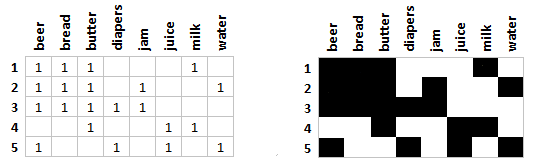
\includegraphics{figures/05/example_bitmap.png}
\caption{Bitmapa przygotowana dla danych z tablicy~\ref{example:data}}\label{rys:example_bitmap}
\end{figure}

Procedura $\proc{Build bitmap}$ tworzy bitmapę na podstawie zestawu transakcji z bazy danych.

\begin{codebox}
	\Procname{$\proc{Build bitmap}$}
		\li \For \textbf{each} element $e \in I$ 
		\li \Do
			\li \For \textbf{each} transakcja $T \in DB$
					\li \Do 
						\If $e \in T$
						\li \Then
							\textbf{set pixel} $(e_{id}, T_{id}) \gets true$\label{li:set_bitmap}\CommentSymbol element występuje w transakcji
						\End
					\End
		\End
\end{codebox}

Jak łatwo zauważyć w procedurze $\proc{Build bitmap}$ dokonywany jest jednokrotny skan wszystkich transakcji, a także wszystkich transakcji - na tej podstawie budowana jest "pionowa" bitmapa - w tym wypadku "pionowa" znaczy, że każdy wiersz reprezentuje jedną transakcję z bazy, natomiast każda kolumna reprezentuje element ze zbioru elementów $I$.

W tym miejscu wymaganym jest także zastosowanie \emph{mostu} (\english{bridge}) pomiędzy obliczeniami na CUDA oraz przetwarzaniem logiki biznesowej w C\# - należało przyjąć język identyfikcji poszczególnych elementów. Źródła danych stosują z reguły identyfikatory - dlatego też zdecydowano się za ich pomocą identyfikować poszczególne elementy. W przypadku gdy źródło danych nie wspierałoby identyfikatorów liczbowych, możliwe jest wprowadzenie takowych na etapie wczytywania danych - co powinno być odpowiednio obsłużone przez importery daanych wejściowych.

Przykładowy fragment bitmapy zbudowanej dla danych, na których oparte zostały eksperymenty został zaprezentowany na rysunku~\ref{rys:data_1}.

\begin{figure}[ht]
\centering
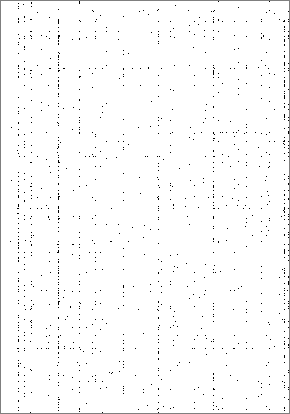
\includegraphics{figures/05/data_1.png}
\caption{Fragment bitmapy z transakcjami}\label{rys:data_1}
\end{figure}

\subsection{Ograniczenie bazy danych}\label{sec:ograniczenie}

Jak łatwo zauważyć na rysunku~\ref{rys:data_1}, gdzie czarnym kolorem zaznaczone są wystąpienia elementu w danej transakcji (biały to ich brak), bitmapa ta jest dość "rzadka", tj. zdecydowanie mniej jest miejsc czarnych niż białych. Oznacza to, że już na tym etapie możliwe jest odrzucenie pewnych elementów, które na pewno nie spełniają wymagań w stosunku do $minsup$.


\begin{codebox}
	\Procname{$\proc{Limit bitmap}$}
		\li \For \textbf{each} kolumna $\id{c} \in bitmap$ \textbf{parallel}
		\li \Do
			\li $\id{sup_c} \gets$ $\frac{\id{wystapienia}}{\id{transakcje}}$
				\li \If $sup_c < minsup$
					\li \Then
						\textbf{delete} kolumna $\id{c}$
					\End
		\End
\end{codebox}

Procedura $\proc{Limit bitmap}$ dokonuje analizy bitmapy zliczając wystąpienia danego elementu w transakcjach. Następnie oblicza wartość $sup_c$, czyli wsparcie dla danego elmentu. Jeśli jego wsparcie jest mniejsze niż minimalne wsparcie $minsup$, to dana kolumna jest usuwana z bitmapy - ponieważ element nie będzie brany pod uwagę w dalszej analizie. Dzięki tej procedurze ograniczona zostaje bitmapa, dzięki czemu możliwa jest szybsza komunikacja pomiędzy CPU a GPU.

\subsection{Generowanie zbiorów częstych}\label{capriori:gen}

Łatwo zauważyć, że ograniczona w punkcie~\ref{sec:ograniczenie} bitmapa składa się wyłącznie z jednoelementowych zbiorów częstych. Na tej podstawie można generować zbiory o krotnościach większych niż $1$. W każdym kolejnym kroku generowane są zbiory częste na podstawie zbiorów wygenerowanych w kroku poprzednim, a proces ten jest kontynuowany do momentu aż nie zostaną znalezione żadne zbiory częste.

Procedura \proc{Cuda Frequent Set Generation} przedstawia pseudokod realizujący opisywany w tym rozdziale algorytm generowania zbiorów częstych.

\begin{codebox}
	\Procname{$\proc{Cuda Frequent Set Generation}$}\label{apriori:listing}
	\li $\id{L_1} \gets \lbrace 1$-zbiory częste - czyli elementy z ograniczonej bitmapy $\rbrace$
		\li \For $(k = 2; \id{L_{k-1}} \neq \emptyset; k++)$
		\li \Do
			 $\id{C_k} \gets aprioriGen(\id{L_{k-1}})$
			\li \For \textbf{each} kandydat $c \in \id{C_k}$ \textbf{parallel}
			\li \Do
					\li \For \textbf{each} transakcja $t \in \id{DB}$
					\li \If $c \subseteq t$
					\li \Then
						\Do c.count++
						\End
					\End
				\End
			\li $L_k \gets \lbrace c \in C_k | c.count \geq minsup \rbrace$	
		\End
	\li Answer $\gets \bigcup_k L_k $
\end{codebox}

Należy podkreślić, że w celu bardziej wydajnej implentacji procedury $\proc{Cuda Frequent Set Generation}$ dokonana została transpozycja macierzy (bitmapy) wystąpień elementów w transakcjach - $bitmapa^T$ powstała z $bitmapy$ poprzez zamianę jej wierszy na kolumny i kolumn na wiersze. 

W wyniku tej operacji możliwe było wydajne zaimplementowanie wspomnianej procedury bez konieczności zapewniania semaforów przy dostępie do pamięci.


\paragraph{Procedura cudaAprioriGen\label{sec:cudaAprioriGen}}
Procedura $\id{cudaAprioriGen}$ reprezentuje proces twórzenia zbiorów $k-$ elementowych zbiorów kandydatów na podstawie zbiorów wejściowych $(k-1)$-elementowych.

Jak łatwo zauważyć wynikiem działania $\proc{Cuda Join Step}$ są zbiory $k$-elementowe, które powstały na podstawie zbiorów wejściowych $L_{k-1}$ o licznościach równych $k-1$, a ich zawartość różni się tylko jednym elementem - ostatnim. Ważnym faktem jest to, iż elementy w zbiorach są uporządkowane leksykograficzne, co wykorzystywane jest w implementacji tej procedury.

\begin{codebox}
	\Procname{$\proc{Cuda Join Step}$}
	\li \textbf{insert into} $C_k$
	\li \textbf{select} p.item$_1$, p.item$_2$, \dots, p.item$_{k-1}$, q.item$_{k-1}$ \textbf{parallel}
	\li \textbf{from} $L_{k-1}$ p, $L_{k-1}$ q
	\li \textbf{where} p.item$_1 = $ q.item$_1$, \dots, p.item$_{k-2}$ = q.item$_{k-2}$, p.item$_{k-1}$ $<$ q.item$_{k-1}$
\end{codebox}

Warto zauważyć, że $\proc{Cuda Join Step}$ jest ekwiwalentem rozszerzania zbioru $L_{k-1}$ każdym elementem zbioru elementów $I$, a następnie kasowania tych $(k)$-zbiorów otrzymanych przez dodanie $(k)$-tego elementu, który nie był w $L_{k-1}$. 

Warunek p.item$_{k-1}$ $<$ q.item$_{k-1}$ zapewnia, że nie będą generowane duplikaty. Dlatego też po etapie łączenia zachodzi zależność $C_k \supseteq L_k$.

Podobnie, jak w przypadku algorytmu równoległego implementowanego na CPU opisanego w części~\ref{sec:papriori}, algorytm CudaApriori nie implementuje etapu obcinania zbiorów, bazując na obserwacji, że zbiorów tych będzie stosunkowo niewiele, a koszt pamięciowy tej operacji byłby zbyt duży.

\subsection{Generowanie reguł asocjacyjnych}
Po zakończeniu pierwszego etapu algorytm przystępuje do drugiego, czyli do budowania reguł asocjacyjnych na podstawie odkrytych zbiorów częstych. Podobnie, jak w~\cite{Apriori:Main} algorytm będący przedmiotem analizy niniejszej pracy, generuje wszystkie możliwe reguły asocjacyjne dla zadanego zbioru.

Aby wygenerować reguły, dla każdego zbioru częstego $l$ znajdowane są niepuste podzbiory - podzbiór taki oznaczony jest jako $a$. Dla takich oznaczeń wygenerowna zostanie reguła $a \Rightarrow (l-a)$, jeżeli spełniona jest nierówność $\frac{support(l)}{support(a)} \geq minconf$.

Procedura~\proc{Generate Frequent Itemsets} prezentuje generowanie reguł asocjacyjnych na podstawie odkrytych $k$-zbiorów częstych $l_k$ będących elementami zbioru $L_k$ ($l_k \in L_k$).

\begin{codebox}
	\Procname{$\proc{Generate Frequent Itemsets}$}
		\li \For \textbf{each} zbiór częsty $l_k$, $k \geq 2$ \textbf{parallel}
		\li \Do
			\textbf{call} genrules($l_k$, $l_k$)
			\End
		\End
\end{codebox}

Widać, że w implementacji algorytmu użyta została metoda $\proc{Genrules}$, która powstała w ramach algorytmu Apriori, opisanego w części~\ref{sec:genrules} niniejszej pracy. Postanowiono, że zrównoleglenie obliczeń wykonane zostanie na wyższym poziomie - tj. na poziomie poszczególnych zbiorów częstych, co znacząco przyspiesza operacje pamięci potrzebne na skopiowanie danych dla każdego zbioru zajęło by zbyt dużo czasu. Dlatego też pominięto opis wspomnianej procedury.